% !TeX spellcheck = en_GB
\documentclass[11pt]{article}

\usepackage[type1]{libertine}
\usepackage[a4paper]{geometry}
\usepackage{amsmath, amsthm, amssymb} 
\usepackage{parskip}
\usepackage{tabularx}
\usepackage[english]{babel}
\usepackage{enumitem}
\usepackage{gensymb}
\usepackage{bm}
\usepackage{graphicx}
\usepackage{xcolor}
\usepackage{float}
\usepackage{wrapfig}
\usepackage{cancel}
\usepackage{multicol}

\newenvironment{multicolFigure}
{\par\medskip\noindent\minipage{\linewidth}}
{\endminipage\par\medskip}
% https://tex.stackexchange.com/questions/12262/multicol-and-figures

\newcommand{\uvec}[1]{\boldsymbol{\hat{\textbf{#1}}}}
\newcommand{\solution}[1]{\textbf{Solution: } #1 \hspace{5mm}}

\title{Worked Solution to Kinematics Problem Set\\{{\small Questions originally compiled by Tan Jing Long, 2016}}}
\author{Sun Yudong\\Hwa Chong Institution}

\begin{document}
	\maketitle
	\section*{Warm-up Questions}
	\begin{multicols}{2}
		\begin{enumerate}
			\item \solution{B}
			\begin{align*}
				v^2 &= u^2 + 2as \\
				s &= \frac{v^2 - u^2}{2a} \\
				&= \frac{(24)^2 - (4.0)^2}{2(3.0)} \\
				&= 93 ~\text{m}
			\end{align*}
			\item \solution{B}
			\begin{align*}
				s = ut - \frac{1}{2}gt^2 &= 0 \\
				t\left(u-\frac{1}{2}gt\right) &= 0 \\
				\because t \neq 0 \therefore t &= \frac{2u}{g} \\
				\Delta t &= \frac{2(30)}{9.81}(\sin 40\degree-\sin 50\degree) \\
				&= -0.754 \approx -\frac{3}{4}
			\end{align*}
			\item \solution{B}
			\begin{align*}
				\arctan \left(\frac{v_{R_y}}{v_{R_x}}\right) &= \arctan \left(\frac{200}{150}\right) \\
				\frac{v_{R_y}}{v_{R_x}} &= \frac{4}{3} \\
				\frac{u_s \cos \theta}{-u_s \sin \theta + v_r} &= \frac{4}{3} \\
				3u_s\cos \theta &= -4u_s\sin\theta + 4v_r \\
				u_s(3\cos\theta + 4\sin\theta) &= 4v_r \\
				u_s &= \frac{4v_r}{3\cos\theta + 4\sin\theta} \\
				&= \frac{4(5.00)}{3\cos 45\degree + 4\sin 45\degree} \\
				&= 4.04 ~\text{km/h}
 			\end{align*}
		\end{enumerate}
	\end{multicols}
	\section*{Conceptual Questions}
	\begin{enumerate}
		\setcounter{enumi}{3}
		\item \solution{B} Velocity of the 2 balls are not the same since \textit{B} is faster than \textit{A}. Displacement of the 2 balls are the same since they are at the same parallel distance away from the start point. The only acceleration on the balls is provided by gravity, which is the same for both balls.
		\item \solution{B} Assuming the rain is uniform, the number of raindrops per unit area does not change regardless of what angle the rain is hitting the ground. Since the cross-sectional area of the cylinder is constant, the time it takes to fill the cylinder will also be constant. 
		\item \solution{C} The initial acceleration on the ball $a = g\sin\theta$ increases in the following order $a_\text{\textit{I}}<a_\text{\textit{II}}<a_\text{\textit{III}}$. Thus, over the course of the whole path, the average velocity of the balls increases in the following order $\left<v\right>_\text{\textit{I}}<\left<v\right>_\text{\textit{II}}<\left<v\right>_\text{\textit{III}}$. Thus, ball \textit{III} will take the least amount of time.
		\item \solution{B} At the top of the flight, the ball comes to an instantaneous rest ($\vec{v}=0$). Thus, at the top of the flight, the frictional force is zero, and the net force on the rock is equal the force of gravity $\implies \vec{a_{net}} = \vec{g}$. 
		\item \solution{C}
		\begin{enumerate}[label={[\arabic*]}]
			\item When going up, air resistance acts in the same direction as gravity. On the way down, air resistance acts in the opposite direction as gravity. $F_{up} > F_{down}$. Thus, the paper slows down faster than it speeds up. 
			\item The distance going up and coming down is the same since the paper returns to the point there it is projected.
			\item The paper comes to an instantaneous rest at the top of its trajectory before travelling in the opposite direction when going back down.
			\item Let $u$ be the initial speed, and $v$ be the final speed when the ball comes back.
			\begin{align*}
				\text{Going up: } &0^2 = u^2+2a_{up}S &\implies u^2 &= -2a_{up}S\\
				\text{Going down: } &v^2=0^2+2a_{down}S &\implies v^2 &= 2a_{down}S  \\
				\because S = \text{constant} \therefore ~&u \propto \sqrt{a_{up}} ~~\text{and}~~v \propto \sqrt{a_{down}}
			\end{align*}
			As explained in [1], $F_{up} > F_{down}$. Thus $a_{up} > a_{down}$, which means that $u > v$.
		\end{enumerate}
		\pagebreak
		\item \solution{E} Although it is true that the time of flight is usually determined  solely by the vertical component of the flight. The trick in this question is that Superman is launching the balls off a very tall building \textbf{\textit{on Earth}}, which is a sphere. Thus, if the horizontal velocity of the ball is high enough, it is possible for the red ball to strike the ground later than the blue ball. 
		\begin{figure}[h]
			\centering
			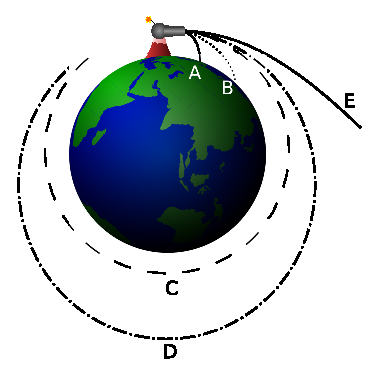
\includegraphics[height=4cm]{Newton_Cannon.eps}
			\caption{Newton's Cannon}
		\end{figure}
	\end{enumerate}
	\section*{Worked Questions}
	\begin{multicols}{2}
		\begin{enumerate}
			\setcounter{enumi}{9}
			\item \solution{C}
			\begin{align*}
				s &= vt - \frac{1}{2}at^2 \\
				&= - \frac{1}{2}(-g)t^2 \\
				&= \frac{g}{2}\left(\frac{1}{n}\right)^2 ~~~~\because t=\frac{1}{n} \\
				&= \frac{g}{2n^2}
			\end{align*}
			\item \solution{B} Smallest angle that the final velocity of an impacting fragment makes with the horizontal is when the fragment is shot horizontally out.
			\begin{align*}
				v_y^2 &= 2as = 2gh\\
				\theta &= \arctan\left(\frac{v_y}{v_x}\right) \\
				&= \arctan\left(\frac{\sqrt{2gh}}{v}\right)
			\end{align*}
			\columnbreak
			\item \solution{C} Since the object falls from rest, $S \propto t^2$. Thus total distance fallen has the ratio $1:4:9$, resulting in the ratio of the distance fallen in each second as $1:3:5$
			\item \solution{E} Since we want the time taken to be at the minimum, we need to find a situation in which the average velocity of the train is the highest:
			\begin{multicolFigure}
				\centering
				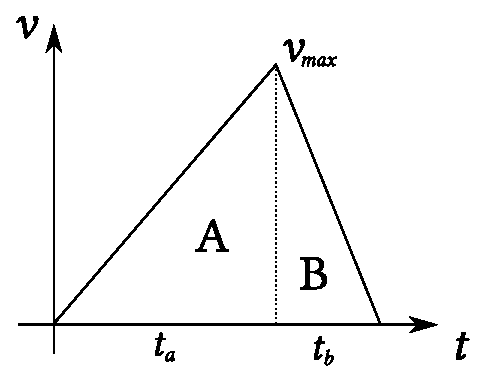
\includegraphics[width=0.60\linewidth]{train.eps}
			\end{multicolFigure}
			\begin{align*}
				v_{max} = a_at_a &= a_bt_b \\
				\implies t_b &= \frac{a_a}{a_b}t_a = \frac{1}{5}t_a\\
			\end{align*}
			Using area under the graph\footnote{You can use the kinematics formulae directly also.}: 
			\begin{align*}
			S &= S_A + S_B \\
			&= \frac{1}{2}(t_a + t_b)(v_{max}) \\
			&= \frac{1}{2}\left(t_a + \frac{1}{5}t_a\right)(a_at_a) \\
			&= \frac{1}{2}\left(\frac{6}{5}t_a\right)a_at_a \\
			&= \frac{3}{5}t_a^2a_a \\
			\implies t_a &= \sqrt{\frac{5S}{3a_a}} \\
			t_{total} &= \frac{6}{5}t_a \\
			&= \frac{6}{5}\sqrt{\frac{5(2\times 10^3)}{3(20\times 10^{-2})}} \\
			&= 154.9 ~\text{s}
			\end{align*}
			
			\item \solution{B}
			\begin{align*}
				\text{Time taken to finish} &= \frac{7.5}{15} = \frac{1}{2} ~\text{h} \\
				\text{Distance travelled} &= \frac{1}{2} (30) = 15 ~\text{km}
			\end{align*}
			\vspace{10cm}
			
			\item \solution{$\displaystyle \frac{8H}{\Delta T_L^2-\Delta T_H^2}$}
			\begin{align*}
				\text{Using } s = ut + \frac{1}{2}at^2,\\
				\text{At both levels: } 0 &= u_i\Delta T_i - \frac{1}{2}g\Delta T_i^2 \\
				u_i\Delta T_i &= \frac{1}{2}g\Delta T_i^2 \\
				u_i &= \frac{1}{2}g\Delta T_i \\
				\text{Using } v^2 = u^2 +2as, \\
				\left(\frac{1}{2}g\Delta T_H\right)^2 &= \left(\frac{1}{2}g\Delta T_L\right)^2 - 2gH \\
				2\cancel{g}H &= \frac{1}{4}g^{\cancel{2}}\left(\Delta T_L^2-\Delta T_H^2\right) \\
				g &= \frac{8H}{\Delta T_L^2-\Delta T_H^2}
			\end{align*}
			
			\item \solution{A}
			\begin{align*}
				S_x = vt ~~&\text{and}~~ S_y = \frac{1}{2}gt^2 \\
				\text{When it hits,} ~\tan\theta &= \frac{S_y}{S_x} = \frac{0.5gt^{\cancel{2}}}{v\cancel{t}} \\ &= \frac{g}{2v}t \\
				\implies t &= \frac{2v\tan\theta}{g} \\
				\tan \alpha = \frac{v_y}{v_x} = \frac{gt}{v} &= \frac{\cancel{g}}{\cancel{v}}\left(\frac{2\cancel{v}\tan\theta}{\cancel{g}}\right) = 2\tan\theta
			\end{align*}
			$\implies \alpha$ is independent of $v$ 
		\end{enumerate}
	\end{multicols}
\end{document}